\documentclass[a4paper, fleqn]{article}

%% Language and font encodings
\usepackage[english]{babel}
\usepackage[utf8x]{inputenc}
\usepackage[T1]{fontenc}

%% Sets page size and margins
\usepackage[a4paper,top=3cm,bottom=2cm,left=3cm,right=3cm,marginparwidth=1.75cm]{geometry}

\usepackage{graphicx}
\usepackage{float}
\usepackage{tikz}
\usetikzlibrary{arrows, automata, shapes, positioning}

\title{Architecture of mcrl2ide}
\author{Olav Bunte}

\begin{document}
\maketitle


\section{Introduction}
The tool \texttt{mcrl2ide} is a graphical tool aimed at users unfamiliar with the mCRL2 toolset to help them use the basic functionalities of the toolset. It is built using the Qt framework and it consists of 9 header files, 10 source files, two ui files, one qrc file and a folder of icons. There are 9 modules, consisting of one header and one source file. This leaves one source file, namely \texttt{main.cpp}, which is the entry point of the application. The two ui files, \texttt{addeditpropertydialog.ui} and \texttt{findandreplacedialog.ui} are created using Qt Creator and describe the widget layout of the add/edit property dialog and the find and replace dialog respectively. The qrc file describes what resources (icons) are used by the tool.


\section{Modules}
There are 9 modules in \texttt{mcrl2ide}: MainWindow, ConsoleDock, PropertiesDock, PropertyWidget, FindAndReplaceDialog, AddEditPropertyDialog, CodeEditor, ProcessSystem and FileSystem. See figure \ref{classdepgraph} for the dependencies between these modules.

\begin{figure}[t]
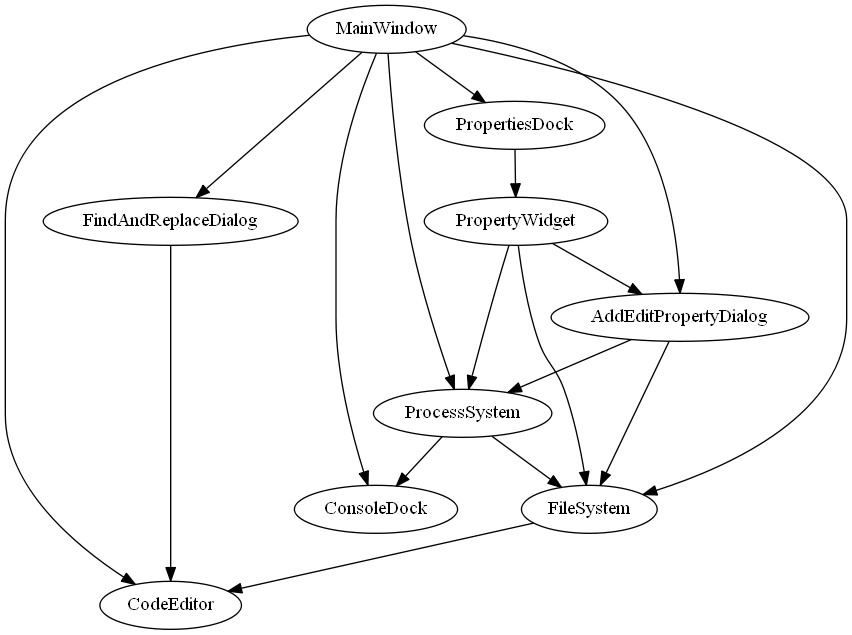
\includegraphics[width=\textwidth]{classDependencyGraph.png}
\caption{Dependency graph of the modules in \texttt{mcrl2ide}. A full arrow from module A to module B means that A creates B or that A uses functions defined on B.}
\label{classdepgraph}
\end{figure}

\subsubsection*{MainWindow}
MainWindow is (after main.cpp) the entry point of the application and it defines the main window. As MainWindow is the entry point, it creates instances of almost all other modules and passes them on when necessary.\\
It also creates the menu bar and and the toolbar, including the actions that correspond to all options on the menu bar and the toolbar. For every action a method is implemented that is called when the action is triggered, which (often) then delegates handling this action to another module (FileSystem for file related actions, ProcessSystem for tool related actions).\\
Whenever the state changes, MainWindow takes care of the changes in the main window. For instance, when a project has been opened the title changes and properties are added via PropertiesDock and when a process is running "start process" buttons change to "abort buttons".

\subsubsection*{ConsoleDock}
ConsoleDock defines the QDockWidget that prints console output, by default located at the bottom. It is mainly used by ProcessSystem to show progress of a running process and output generated by the tools. It has one tab for each process type: parsing, simulation, state space generation and verification.

\subsubsection*{PropertiesDock}
PropertiesDock defines the QDockWidget that holds defined properties, by default located on the right. Whenever a new property is defined, the PropertiesDock creates the corresponding PropertyWidget and lays it out in the dock.

\subsubsection*{PropertyWidget}
PropertyWidget defines the widget that holds a property. It creates the buttons and corresponding actions that appear on the PropertyWidget. Similar to MainWindow, it has a method for each such action that is called when the action is triggered, which (often) delegates handling this action to another module. It also creates an AddEditPropertyDialog that is used when editing a property.

\subsubsection*{FindAndReplaceDialog}
FindAndReplaceDialog defines the dialog that is used to find and/or replace strings in the specification editor. It also implements the functionality to do so. It creates a code editor for entering a mu-calculus formula. It uses ProcessSystem to parse the entered property and FileSystem to save the property.

\subsubsection*{AddEditPropertyDialog}
AddEditPropertyDialog defines the dialog that is used to add a property to the project (add-variant) or to edit a previously defined property (edit-variant).

\subsubsection*{CodeEditor}
CodeEditor defines a text editor for mcrl2 specifications or mu-calculus formulas. It creates a widget for line numbers and it implements basic text editor functionalities such as selecting, copying, cutting, pasting, undoing, redoing, zooming and syntax highlighting.

\subsubsection*{ProcessSystem}
ProcessSystem handles all things related to tools. It creates and runs processes for any tool action that can be required, such as parsing, creating a simulation, creating and visualising a (reduced) state space and checking a property. It has one ProcessThread for each process type, which uses queues to make sure that one process of that process type runs at a time. How this works will be explained in more detail in section \ref{secprocesses}.

\subsubsection*{FileSystem}
FileSystem handles all thing related to files, such as creating, opening and saving files. It also contains most of the application state such as project information.


\subsection{Modules during application lifetime}
During the lifetime of the application, there is only one instance of the modules MainWindow, ConsoleDock, PropertiesDock, FindAndReplaceDialog, ProcessSystem and FileSystem. The number of instances of PropertyWidget can change, depending on how many properties there are defined in a current project. There is one instance of the add-variant of AddEditPropertyDialog (used by MainWindow) and there is one instance of the edit-variant of AddEditPropertyDialog for every PropertyWidget. There is one instance of CodeEditor used by MainWindow and there is one instance of CodeEditor per AddEditPropertyDialog.\\
The user can only directly change the number of instances of PropertyWidget. All other changes in number of instances are caused (directly or indirectly) by change in the number of instances of PropertyWidget.


\subsection{Signals}
Apart from invoking a method synchronously, in Qt it is also possible to invoke methods asynchronously using signals. A signal can be connected to a method (slot) and when this signal is emitted, a new thread will spawn for every slot it is connected to which then executes the method. The (main) thread that has emitted the signal simply continues right after emission. This is especially useful for changing the UI when the state changes. In \texttt{mcrl2ide} this is also used for handling processes. See figure \ref{classdepgraphwithsignals} for the dependency diagram which also includes signals between modules.

\begin{figure}[b!]
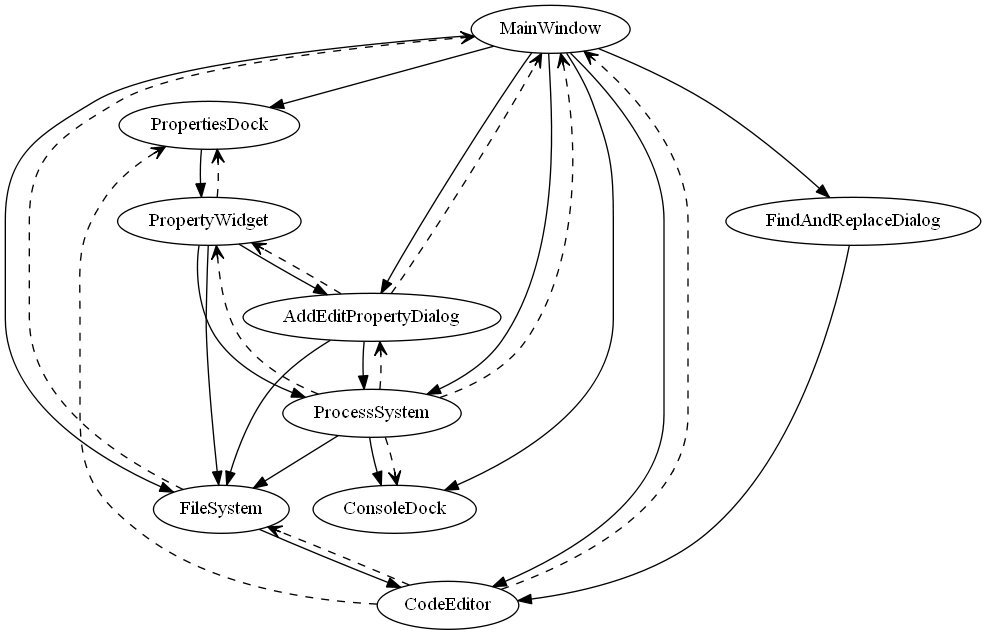
\includegraphics[width=\textwidth]{classDependencyGraphWithSignals.png}
\caption{Dependency graph of the modules in \texttt{mcrl2ide} including signals. A full arrow from module A to module B means that A creates B or that A uses functions defined on B. A striped arrow from module A to B means that A can send signals to a slot on B.}
\label{classdepgraphwithsignals}
\end{figure}


\section{Activity}
In this section we will explain in more detail what activity happens in the background when the user interacts with \texttt{mcrl2ide}.

\subsection{Processes}
\label{secprocesses}
As mentioned before, there are 4 process types (parsing, simulation, state space generation and verification) and each has its own ProcessThread. The reason each has its own ProcessThread is that this allows processes of different process types to run in parallel. Whenever the user invokes an action that needs tools to run, a process is created. A process consists of subprocesses (QProcesses), each of which corresponds to a single run of a single tool. The subprocesses are parsemcrl2 (which uses \texttt{mcrl22lps}), mcrl22lps, lpsxsim, lps2lts, ltsconvert, ltsgraph, parsemcf (which uses \texttt{lps2pbes}), lps2pbes and pbessolve. When a process is created, all corresponding subprocesses are created. Also all data that is needed by the subprocesses such as filepaths is fixed at the creation of the process. After a process has been created, it is added to the queue of the corresponding ProcessThread.\\
A ProcessThread makes sure that queued processes are run in parallel with the main thread and it can be in two states: waiting or running. If it is in state waiting, there is no process running that corresponds to this thread and there is no process in the queue. If it is in state running there is a process running that corresponds to this thread. While it is in a state it is blocked until it receives a signal from outside. See figure \ref{procthread} for the behaviour of a ProcessThread. Note that a ProcessThread only regulates the (running of) processes, it does not execute them itself.\\
After a subprocess has finished, a "finished" signal is sent that activates a slot that handles starting the next subprocess. In case the next subprocess creates an output file, it is first checked whether there already exists an up to date output file. If this is the case, the next subprocess does not need to be run and we simply emit its "finished" signal. If there is no up to date output file, we start the next subprocess.\\
When a process has finished, it emits its "finished" signal. The point at which a process finishes differs per process. Processes of type simulation or state space generation end with a subprocess that runs a graphical tool (lpsxsim, ltsgraph). These already emit their "finished" signal just before starting the last subprocess to allow viewing multiple instances (for instance to see different reduced LTSs next to each other). Processes of type parsing or verification emit their "finished" signal after the last subprocess has finished. The result of these processes (valid/invalid or true/false) are stored in ProcessSystem and can be retrieved when necessary.\\
Processes may be aborted by the user. When this happens, it is first checked whether this process is running. If this is the case, the corresponding running subprocess is muffled (so that it does not activate the next subprocess) and then killed. If the subprocess is not running but in a queue, it is removed from the queue. In both cases the "finished" signal of the process is emitted afterwards to let the corresponding ProcessThread continue the next process if it was running the aborted process and to change the UI.

\begin{figure}[b!]
\centering
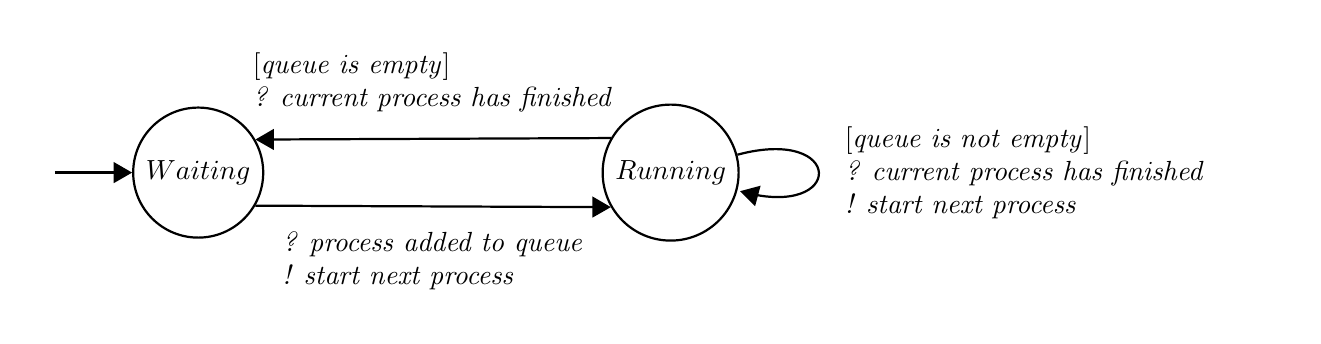
\begin{tikzpicture}[->, >=triangle 60, auto, swap, thick, ellipse, align=left]
	
	\node			(init)	at	(-2, 0)	{};
	\node[state]	(W)		at	(0, 0)	{$Waiting$};
	\node[state]	(R)		at	(6, 0)	{$Running$};
	\node			(label)	at	(10.5, 0)	{[\textit{queue is not empty}] \\ \textit{? current process has finished} \\ \textit{! start next process}};
 
	\path 	(init)	edge			node	{}	(W)
			(W.330)	edge			node	{\textit{? process added to queue} \\ \textit{! start next process}}	(R.210)
			(R.150)	edge			node	{[\textit{queue is empty}] \\ \textit{? current process has finished}}	(W.30)
			(R)	edge[loop right]	node	{}	(R);
			
\end{tikzpicture}
\caption{The behaviour of a ProcessThread. An edge label can consist of three parts: a guard surrounded by [ ], an incoming signal preceded by \textit{?} and an action executed by the ProcessThread preceded by \textit{!}.}
\label{procthread}
\end{figure}


\subsection{User input}
TODO activity diagrams/explanations of what happens after user input

























\end{document}